\documentclass[10pt,aspectratio=169]{beamer}

% ============================================================================
% THEME AND COLORS
% ============================================================================
% Modern, clean theme
\usetheme{Madrid}
\useinnertheme{rounded}
\useoutertheme{infolines}

% Fix frame numbering
\setbeamertemplate{footline}
{
  \leavevmode%
  \hbox{%
  \begin{beamercolorbox}[wd=.333333\paperwidth,ht=2.25ex,dp=1ex,center]{author in head/foot}%
    \usebeamerfont{author in head/foot}\insertshortauthor~~\beamer@ifempty{\insertshortinstitute}{}{(\insertshortinstitute)}
  \end{beamercolorbox}%
  \begin{beamercolorbox}[wd=.333333\paperwidth,ht=2.25ex,dp=1ex,center]{title in head/foot}%
    \usebeamerfont{title in head/foot}\insertshorttitle
  \end{beamercolorbox}%
  \begin{beamercolorbox}[wd=.333333\paperwidth,ht=2.25ex,dp=1ex,right]{date in head/foot}%
    \usebeamerfont{date in head/foot}\insertshortdate{}\hspace*{2em}
    \insertframenumber{} / \inserttotalframenumber\hspace*{2ex}
  \end{beamercolorbox}}%
  \vskip0pt%
}

% Custom color scheme - deep blue and purple tones (scientific but vibrant)
\definecolor{primaryblue}{RGB}{30,64,175}      % Deep scientific blue
\definecolor{accentpurple}{RGB}{109,40,217}    % Vibrant purple accent
\definecolor{lightblue}{RGB}{147,197,253}      % Light blue for highlights
\definecolor{warmorange}{RGB}{251,146,60}      % Warm orange for emphasis
\definecolor{softgray}{RGB}{229,231,235}       % Soft gray background
\definecolor{darkgray}{RGB}{55,65,81}          % Dark gray for text

\setbeamercolor{structure}{fg=primaryblue}
\setbeamercolor{title}{fg=primaryblue}
\setbeamercolor{frametitle}{fg=primaryblue}
\setbeamercolor{block title}{bg=primaryblue,fg=white}
\setbeamercolor{block body}{bg=softgray}
\setbeamercolor{alerted text}{fg=accentpurple}
\setbeamercolor{example text}{fg=primaryblue}

% ============================================================================
% PACKAGES
% ============================================================================
\usepackage[T1]{fontenc}
\usepackage[utf8]{inputenc}
\usepackage{lmodern}
\usepackage{amsmath,amssymb,amsthm}
\usepackage{bm}                    % Bold math
\usepackage{mathtools}             % Enhanced math
% \usepackage{physics}               % Physics-style notation (\qty, etc.) - not used
% \usepackage{siunitx}               % Units - not used
\usepackage{graphicx}
\usepackage{booktabs}              % Better tables
\usepackage{xcolor}
\usepackage{tikz}
\usetikzlibrary{shapes,arrows,positioning,calc}
% \usepackage{fontawesome5}          % Icons - not installed
% Define simple replacements for icons
\newcommand{\faDna}{$\otimes$}
\newcommand{\faChartLine}{$\nearrow$}
\newcommand{\faCode}{$\langle\rangle$}
\newcommand{\faCheckCircle}{$\checkmark$}
\newcommand{\faGlobe}{$\odot$}
\newcommand{\faHeartbeat}{$\heartsuit$}
\newcommand{\faFlask}{$\star$}
\newcommand{\faEnvelope}{$\square$}
\newcommand{\faGithub}{$\circ$}

% Math shortcuts for the talk
\newcommand{\aladyn}{\textsc{Aladynoulli}}
\newcommand{\Prob}{\mathbb{P}}
\newcommand{\E}{\mathbb{E}}
\newcommand{\Var}{\text{Var}}
\newcommand{\Cov}{\text{Cov}}

% ============================================================================
% TITLE PAGE INFORMATION
% ============================================================================
\title[Aladynoulli]{\Large \textbf{\aladyn}: \\ 
                    \large A Bayesian Voyage Through the Genome and the EHR}
\subtitle{Methods in Population Genomics 2025}
\author{Sarah M. Urbut}
\institute{Massachusetts General Hospital \& Broad Institute}

% Optional: add date
\date{\today}

% ============================================================================
% CUSTOM COMMANDS FOR CONSISTENT STYLING
% ============================================================================

% Highlight box for key equations
\newcommand{\keyeq}[1]{
    \begin{block}{}
        \centering
        #1
    \end{block}
}

% Beautiful equation display
\newcommand{\beq}[1]{
    \begin{equation*}
        #1
    \end{equation*}
}

% Nice itemize with custom spacing
\newenvironment{niceitemize}
    {\begin{itemize}[<+-|alert@+>]
        \setlength\itemsep{0.5em}}
    {\end{itemize}}

% Theorem/definition environment with custom styling
\newtheorem{idea}{Key Idea}
\theoremstyle{definition}

% Section page formatting
\AtBeginSection[]{
    \begin{frame}[plain]
        \vfill
        \centering
        \begin{beamercolorbox}[sep=8pt,center,shadow=true,rounded=true]{title}
            \usebeamerfont{title}\insertsectionhead\par%
        \end{beamercolorbox}
        \vfill
    \end{frame}
}

% ============================================================================
% PRESENTATION BEGINS
% ============================================================================

\begin{document}

% ----------------------------------------------------------------------------
% TITLE SLIDE
% ----------------------------------------------------------------------------
\begin{frame}[plain]
    \titlepage
    \begin{tikzpicture}[remember picture,overlay]
        \node[anchor=south east, xshift=-1cm, yshift=1cm] at (current page.south east) {
            \textcolor{primaryblue!20}{\faDna \quad \faChartLine \quad \faCode}
        };
    \end{tikzpicture}
\end{frame}

% ----------------------------------------------------------------------------
% SECTION: THE PROBLEM - WHY DO WE NEED THIS?
% ----------------------------------------------------------------------------
\section{Why This Matters}

\begin{frame}{The Problem: Diseases Don't Exist in Isolation}
    \begin{columns}
        \column{0.5\textwidth}
        \begin{block}{Traditional Approach}
            \begin{itemize}
                \item Study one disease at a time
                \item Simple risk factors (age, sex)
                \item Static models
                \item Misses biological complexity
            \end{itemize}
        \end{block}
        
        \column{0.5\textwidth}
        \begin{block}{Reality}
            \begin{itemize}
                \item Diseases \alert{co-occur} in patterns
                \item Shared biological pathways
                \item Risk evolves over lifetime
                \item Need to \textbf{borrow strength} across diseases
            \end{itemize}
        \end{block}
    \end{columns}
    
    \vspace{1em}
    \begin{exampleblock}{Example}
        Metabolic syndrome: Hypertension, Type 2 Diabetes, and Coronary Artery Disease 
        don't appear randomly—they cluster together in time and share genetic basis.
    \end{exampleblock}
\end{frame}

\begin{frame}{The Problem: Time Matters}
    \begin{columns}
        \column{0.5\textwidth}
        \begin{block}{Traditional Models}
            \textbf{Cox Proportional Hazards:}
            \beq{
                h(t | \mathbf{X}) = h_0(t) \exp(\beta^T \mathbf{X})
            }
            \begin{itemize}
                \item Relative risk is \alert{constant over time}
                \item Doesn't capture life course dynamics
                \item When you ask matters!
            \end{itemize}
        \end{block}
        
        \column{0.5\textwidth}
        \begin{block}{Why This Is a Problem}
            \begin{itemize}
                \item Same individual, different ages → different risk
                \item Genetic effects manifest differently across life course
                \item Need dynamic, time-varying models
            \end{itemize}
        \end{block}
    \end{columns}
    
    \vspace{1em}
    \begin{center}
        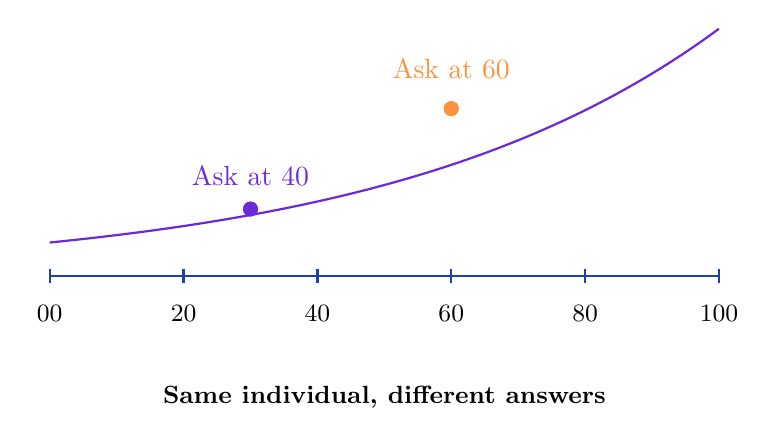
\begin{tikzpicture}[scale=0.85]
            \draw[thick, primaryblue] (0,0) -- (10,0);
            \foreach \x in {0,2,4,6,8,10} {
                \draw[thick, primaryblue] (\x,0.1) -- (\x,-0.1);
                \node[below] at (\x,-0.3) {\small \x0};
            }
            \draw[smooth, thick, accentpurple] 
                plot[domain=0:10,samples=100] (\x,{0.5*exp(0.2*\x)});
            \filldraw[accentpurple] (3,1) circle (3pt);
            \node[above, accentpurple] at (3,1.2) {Ask at 40};
            \filldraw[warmorange] (6,2.5) circle (3pt);
            \node[above, warmorange] at (6,2.8) {Ask at 60};
            \node[below] at (5,-1.5) 
                {\small \textbf{Same individual, different answers}};
        \end{tikzpicture}
    \end{center}
\end{frame}

\begin{frame}{The Problem: Rich Data, Simple Models}
    \begin{block}{What We Have}
        \begin{itemize}
            \item \textbf{Longitudinal EHR}: Diagnoses over time for millions of patients
            \item \textbf{Genetics}: PRS for multiple diseases
            \item \textbf{Complex patterns}: Diseases co-occur, evolve, interact
        \end{itemize}
    \end{block}
    
    \vspace{1em}
    
    \begin{block}{What We Need}
        \begin{enumerate}
            \item \textcolor{accentpurple}{\textbf{Discover latent patterns}} of disease co-occurrence
            \item \textcolor{primaryblue}{\textbf{Model time-varying trajectories}} for individuals
            \item \textcolor{warmorange}{\textbf{Integrate genetics}} to inform individual risk
            \item \textcolor{darkgray}{\textbf{Predict future disease}} while learning biology
        \end{enumerate}
    \end{block}
    
    \vspace{1em}
    \begin{center}
        \Large
        \textcolor{accentpurple}{\textbf{Solution: Bayesian hierarchical model}}
    \end{center}
\end{frame}

\begin{frame}{When You Ask Matters}
    \begin{center}
        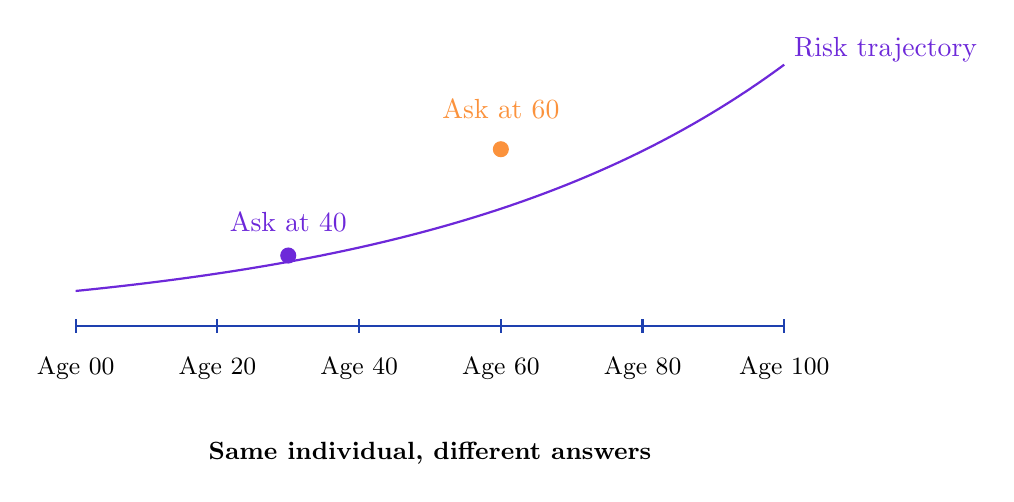
\begin{tikzpicture}[scale=0.9]
            % Timeline
            \draw[thick, primaryblue] (0,0) -- (10,0);
            \foreach \x in {0,2,4,6,8,10} {
                \draw[thick, primaryblue] (\x,0.1) -- (\x,-0.1);
                \node[below] at (\x,-0.3) {\small Age \x0};
            }
            
            % Risk curve
            \draw[smooth, thick, accentpurple] 
                plot[domain=0:10,samples=100] (\x,{0.5*exp(0.2*\x)});
            \node[above right, accentpurple] at (10,3.6) {Risk trajectory};
            
            % Points where question is asked
            \filldraw[accentpurple] (3,1) circle (3pt);
            \node[above, accentpurple] at (3,1.2) {Ask at 40};
            \filldraw[warmorange] (6,2.5) circle (3pt);
            \node[above, warmorange] at (6,2.8) {Ask at 60};
            
            % Labels
            \node[below] at (5,-1.5) 
                {\small \textbf{Same individual, different answers}};
        \end{tikzpicture}
    \end{center}
    
    \vspace{1em}
    \begin{center}
        \textcolor{darkgray}{\textit{The question changes as we move through life}}
    \end{center}
\end{frame}

% ----------------------------------------------------------------------------
% SECTION: BUILDING THE MODEL STEP BY STEP
% ----------------------------------------------------------------------------
\section{Building the Model}

\begin{frame}{Why Bayesian? Natural Framework for This Problem}
    \begin{block}{The Bayesian Philosophy}
        \begin{center}
            \Large
            \[
            \Prob(\text{Model} \mid \text{Data}) \propto 
            \Prob(\text{Data} \mid \text{Model}) \cdot \Prob(\text{Model})
            \]
        \end{center}
    \end{block}
    
    \vspace{1em}
    
    \begin{columns}
        \column{0.33\textwidth}
        \begin{block}{\centering Prior}
            \centering
            \textbf{Population knowledge}\\
            Disease signatures from all patients
            \vspace{0.5em}
            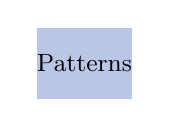
\begin{tikzpicture}[scale=0.6]
                \fill[primaryblue!30] (0,0) rectangle (2,1.5);
                \node at (1,0.75) {\small Patterns};
            \end{tikzpicture}
        \end{block}
        
        \column{0.33\textwidth}
        \begin{block}{\centering Likelihood}
            \centering
            \textbf{Individual data}\\
            This patient's diagnoses over time
            \vspace{0.5em}
            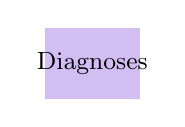
\begin{tikzpicture}[scale=0.6]
                \fill[accentpurple!30] (0,0) rectangle (2,1.5);
                \node at (1,0.75) {\small Diagnoses};
            \end{tikzpicture}
        \end{block}
        
        \column{0.33\textwidth}
        \begin{block}{\centering Posterior}
            \centering
            \textbf{Updated beliefs}\\
            Personalized risk prediction
            \vspace{0.5em}
            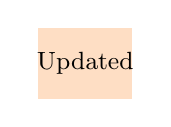
\begin{tikzpicture}[scale=0.6]
                \fill[warmorange!30] (0,0) rectangle (2,1.5);
                \node at (1,0.75) {\small Updated};
            \end{tikzpicture}
        \end{block}
    \end{columns}
    
    \vspace{1em}
    \begin{center}
        \textcolor{accentpurple}{\Large 
        \textbf{Continuous updating as we walk through the lifetime}}
    \end{center}
\end{frame}

\begin{frame}{Step 1: Why Disease Signatures?}
    \begin{block}{The Key Insight}
        Diseases don't occur independently—they cluster in \textbf{signatures} 
        representing shared biological pathways
    \end{block}
    
    \vspace{1em}
    
    \begin{columns}
        \column{0.5\textwidth}
        \begin{exampleblock}{Example Signatures}
            \textbf{Metabolic Signature:}
            \begin{itemize}
                \item Type 2 Diabetes
                \item Hypertension  
                \item Coronary Artery Disease
                \item Obesity
            \end{itemize}
            
            \vspace{0.5em}
            \textbf{Inflammatory Signature:}
            \begin{itemize}
                \item Rheumatoid Arthritis
                \item Inflammatory Bowel Disease
                \item Psoriasis
            \end{itemize}
        \end{exampleblock}
        
        \column{0.5\textwidth}
        \begin{block}{Why This Matters}
            \begin{itemize}
                \item \textbf{Borrow strength}: Learn from similar patients
                \item \textbf{Predict multiple diseases}: Learn signature, predict all
                \item \textbf{Biological interpretation}: Signatures have genetic basis
                \item \textbf{Efficiency}: Don't model each disease separately
            \end{itemize}
        \end{block}
    \end{columns}
    
    \vspace{1em}
    \begin{center}
        \textcolor{primaryblue}{\Large 
        \textbf{Signatures = Latent patterns we discover from the data}}
    \end{center}
\end{frame}

\begin{frame}{Step 2: How Do Signatures Give Us Disease Risk?}
    \begin{block}{The Core Idea: Mixture Model}
        For individual $i$, disease $d$, at time $t$:
        \keyeq{
            \[
            \pi_{i,d,t} = \kappa \cdot \sum_{k=1}^{K} \theta_{i,k,t} \cdot \text{sigmoid}(\phi_{k,d,t})
            \]
        }
    \end{block}
    
    \vspace{1em}
    
    \begin{columns}
        \column{0.5\textwidth}
        \begin{block}{Breaking It Down}
            \begin{itemize}
                \item $\theta_{i,k,t}$: How much does individual $i$ 
                      load on signature $k$ at time $t$?
                      \textcolor{accentpurple}{\textbf{(Individual-specific)}}
                \item $\phi_{k,d,t}$: How strongly is disease $d$ 
                      associated with signature $k$ at time $t$?
                      \textcolor{primaryblue}{\textbf{(Population-level)}}
                \item Multiple signatures can contribute simultaneously!
            \end{itemize}
        \end{block}
        
        \column{0.5\textwidth}
        \begin{alertblock}{Key Innovation}
            This is a \textbf{mixture of probabilities}, not probability of mixture
            
            \vspace{0.5em}
            \textbf{Why this matters:}
            \begin{itemize}
                \item Enables direct risk prediction
                \item Unlike topic models (allocation-based)
                \item Multiple signatures contribute to same disease
            \end{itemize}
        \end{alertblock}
    \end{columns}
\end{frame}

\begin{frame}{Step 3: Why Time-Varying? Signatures Evolve Over Life}
    \begin{block}{Individual Signature Loadings Change Over Time}
        Each individual's association with signatures evolves:
        \beq{
        \theta_{i,k,t} = \frac{\exp(\lambda_{i,k,t})}{\sum_{k'=1}^{K} \exp(\lambda_{i,k',t})}
        }
        \begin{itemize}
            \item Softmax ensures $\sum_k \theta_{i,k,t} = 1$ (proper mixture)
            \item $\lambda_{i,k,t}$ evolves smoothly over time
        \end{itemize}
    \end{block}
    
    \vspace{1em}
    
    \begin{columns}
        \column{0.5\textwidth}
        \begin{block}{Why Time-Varying Matters}
            \begin{itemize}
                \item Young person: Low metabolic signature loading
                \item With age: Metabolic signature increases
                \item This drives changing disease risk over lifetime
            \end{itemize}
        \end{block}
        
        \column{0.5\textwidth}
        \begin{center}
            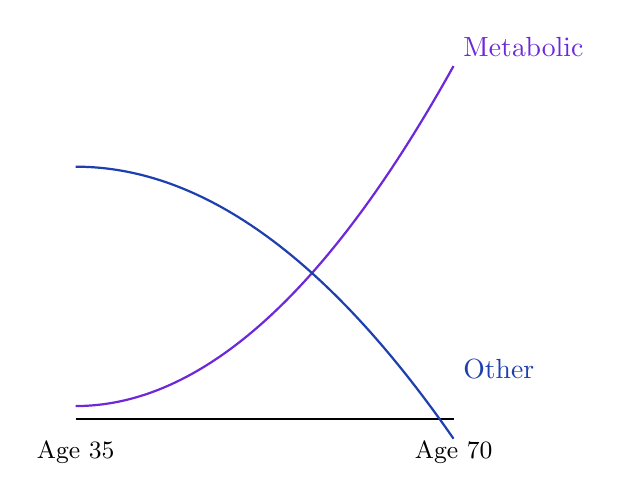
\begin{tikzpicture}[scale=0.8]
                \draw[thick] (0,0) -- (6,0);
                \node[below] at (0,-0.2) {\small Age 35};
                \node[below] at (6,-0.2) {\small Age 70};
                \draw[smooth,thick,accentpurple] 
                    plot[domain=0:6,samples=100] (\x,{0.2 + 0.15*\x*\x});
                \node[above right,accentpurple] at (6,5.6) {Metabolic};
                \draw[smooth,thick,primaryblue] 
                    plot[domain=0:6,samples=100] (\x,{4 - 0.12*\x*\x});
                \node[above right,primaryblue] at (6,0.48) {Other};
            \end{tikzpicture}
        \end{center}
    \end{columns}
\end{frame}

\begin{frame}{Step 4: Why Gaussian Processes? Smooth Temporal Evolution}
    \begin{block}{We Model $\lambda_{i,k,t}$ as a Gaussian Process}
        \beq{
        \lambda_{i,k} \sim \mathcal{GP}\left(\text{mean function}, K_{\lambda}\right)
        }
        
        \textbf{Why GP?}
        \begin{itemize}
            \item Ensures \textbf{smooth trajectories} over time (no wild jumps)
            \item Flexible—can capture any smooth function
            \item Handles irregular observation times
            \item Natural for longitudinal data
        \end{itemize}
    \end{block}
    
    \vspace{1em}
    
    \begin{alertblock}{But what's the mean function?}
        This is where \textbf{genetics comes in!}
    \end{alertblock}
\end{frame}

\begin{frame}{Step 5: Why Genetics? Individual-Level Information}
    \begin{block}{Genetics Modify the Mean Trajectory}
        \beq{
        \lambda_{i,k} \sim \mathcal{GP}\left(r_k + \mathbf{g}_i^{\top}\Gamma_k, K_{\lambda}\right)
        }
    \end{block}
    
    \vspace{1em}
    
    \begin{columns}
        \column{0.5\textwidth}
        \begin{block}{Components}
            \begin{itemize}
                \item $r_k$: Population baseline for signature $k$
                \item $\mathbf{g}_i$: Individual's PRS vector
                \item \textcolor{accentpurple}{$\Gamma_k$}: \textbf{How genetics affect signature $k$} 
                      \textcolor{accentpurple}{\textbf{(learned!)}}
                \item $K_{\lambda}$: Temporal smoothness
            \end{itemize}
        \end{block}
        
        \column{0.5\textwidth}
        \begin{block}{Why This Matters}
            \textbf{High CAD PRS?}
            \begin{itemize}
                \item $\Gamma_{\text{metabolic}}$ tells us how this shifts your metabolic signature trajectory
                \item Higher genetic loading → earlier/stronger signature activation
                \item This provides \textbf{biological interpretation}
            \end{itemize}
        \end{block}
    \end{columns}
    
    \vspace{1em}
    \begin{center}
        \begin{tikzpicture}[scale=0.9]
            \draw[thick] (0,0) -- (6,0);
            \node[below] at (0,-0.2) {\small Age 35};
            \node[below] at (6,-0.2) {\small Age 70};
            \draw[smooth,thick,primaryblue!60] 
                plot[domain=0:6,samples=100] (\x,{1 + 0.1*\x});
            \node[above left,primaryblue!60] at (0,1) {Low PRS};
            \draw[smooth,thick,accentpurple] 
                plot[domain=0:6,samples=100] (\x,{2 + 0.15*\x*\x});
            \node[above right,accentpurple] at (6,7.4) {High PRS};
            \node[below] at (3,-1) {\small \textbf{Genetics shift the entire trajectory}};
        \end{tikzpicture}
    \end{center}
\end{frame}

\begin{frame}{Step 6: Why Population-Level Signatures? Learn from Everyone}
    \begin{block}{Signature-Disease Associations Are Shared}
        \beq{
        \phi_{k,d} \sim \mathcal{GP}\left(\mu_d + \psi_{k,d}, K_{\phi}\right)
        }
        
        \begin{itemize}
            \item $\mu_d$: Disease baseline (population prevalence)
            \item $\psi_{k,d}$: How strongly signature $k$ associates with disease $d$
            \item \textcolor{primaryblue}{\textbf{Learned from all patients}} (not individual-specific)
            \item Time-varying: associations can change over life course
        \end{itemize}
    \end{block}
    
    \vspace{1em}
    
    \begin{columns}
        \column{0.5\textwidth}
        \begin{exampleblock}{Example}
            Metabolic signature strongly associated with:
            \begin{itemize}
                \item T2D: $\psi_{\text{metabolic}, \text{T2D}} = +2.3$
                \item CAD: $\psi_{\text{metabolic}, \text{CAD}} = +1.8$
                \item Cancer: $\psi_{\text{metabolic}, \text{Cancer}} = +0.1$
            \end{itemize}
        \end{exampleblock}
        
        \column{0.5\textwidth}
        \begin{block}{Why This Works}
            \begin{itemize}
                \item \textbf{Borrow strength}: Learn patterns from millions
                \item \textbf{Interpretability}: Signatures have clear meaning
                \item \textbf{Efficiency}: Shared parameters across all individuals
            \end{itemize}
        \end{block}
    \end{columns}
\end{frame}

\begin{frame}{Step 7: Why Bernoulli Survival? Properly Handle Censoring}
    \begin{block}{The Likelihood: Discrete-Time Survival}
        For individual $i$, disease $d$:
        \beq{
        \ell_{i,d} = \sum_{t < E_{i,d}} \log(1 - \pi_{i,d,t}) + 
                     Y_{i,d,t}\log(\pi_{i,d,t}) + 
                     (1-Y_{i,d,t})\log(1-\pi_{i,d,t})
        }
    \end{block}
    
    \vspace{1em}
    
    \begin{columns}
        \column{0.33\textwidth}
        \begin{block}{\centering At Risk}
            Before event time\\
            Person hasn't gotten disease yet\\
            \textcolor{primaryblue}{$(1-\pi)$} terms
        \end{block}
        
        \column{0.33\textwidth}
        \begin{block}{\centering Event}
            Disease occurs at time $t$\\
            \textcolor{accentpurple}{$\log(\pi)$} contribution
        \end{block}
        
        \column{0.33\textwidth}
        \begin{block}{\centering Censored}
            Person leaves study\\
            Last observation at $E_{i,d}$\\
            \textcolor{warmorange}{$(1-\pi)$} at enrollment
        \end{block}
    \end{columns}
    
    \vspace{1em}
    \begin{alertblock}{Why This Matters}
        \textbf{Properly handles censoring} (critical for EHR data!) \\
        and enables \textbf{direct prediction} (unlike topic models)
    \end{alertblock}
\end{frame}

\begin{frame}{Putting It All Together: The Full Model}
    \begin{block}{Individual Disease Probability}
        \keyeq{
            \[
            \pi_{i,d,t} = \kappa \cdot \sum_{k=1}^{K} \theta_{i,k,t} \cdot \text{sigmoid}(\phi_{k,d,t})
            \]
        }
    \end{block}
    
    \vspace{1em}
    
    \begin{columns}
        \column{0.5\textwidth}
        \begin{block}{Individual Component (Time-Varying)}
            \beq{
            \theta_{i,k,t} = \text{softmax}(\lambda_{i,k,t})
            }
            \beq{
            \lambda_{i,k} \sim \mathcal{GP}(r_k + \mathbf{g}_i^{\top}\Gamma_k, K_{\lambda})
            }
        \end{block}
        
        \column{0.5\textwidth}
        \begin{block}{Population Component (Shared)}
            \beq{
            \phi_{k,d} \sim \mathcal{GP}(\mu_d + \psi_{k,d}, K_{\phi})
            }
        \end{block}
    \end{columns}
    
    \vspace{1em}
    \begin{center}
        \Large
        \textcolor{accentpurple}{\textbf{Genetics + Population Patterns + Time = Personalized Risk}}
    \end{center}
\end{frame}

% ----------------------------------------------------------------------------
% SECTION: WALKING THROUGH THE LIFETIME
% ----------------------------------------------------------------------------
\section{Walking Through the Lifetime}

\begin{frame}{The Bayesian Update Cycle in Action}
    \begin{center}
        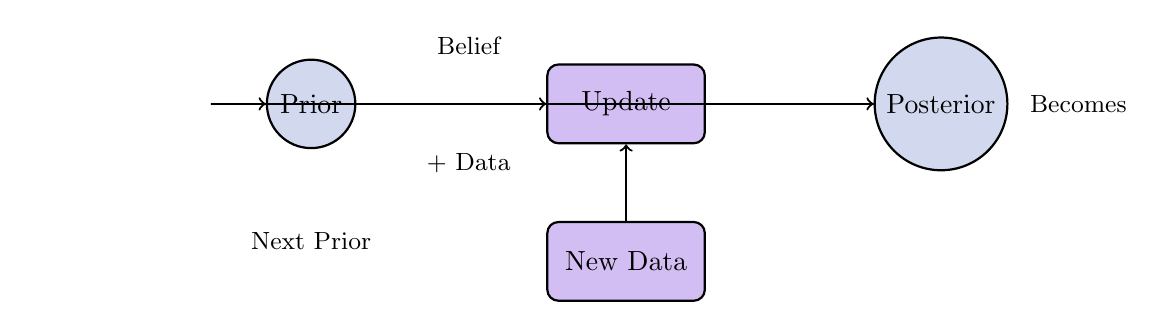
\begin{tikzpicture}[
            node distance=2cm,
            auto,
            thick,
            main node/.style={circle,fill=primaryblue!20,draw,minimum size=1cm},
            update node/.style={rectangle,fill=accentpurple!30,draw,rounded corners,minimum width=2cm,minimum height=1cm}
        ]
            \node[main node] (prior) at (0,0) {Prior};
            \node[update node] (update) at (4,0) {Update};
            \node[main node] (posterior) at (8,0) {Posterior};
            \node[update node] (data) at (4,-2) {New Data};
            
            \draw[->,thick] (prior) -- (update);
            \draw[->,thick] (update) -- (posterior);
            \draw[->,thick] (data) -- (update);
            \draw[->,thick] (posterior) to[out=180,in=180] (prior);
            
            \node[above] at (2,0.5) {\small Belief};
            \node[below] at (2,-0.5) {\small + Data};
            \node[right] at (9,0) {\small Becomes};
            \node[below] at (0,-1.5) {\small Next Prior};
        \end{tikzpicture}
    \end{center}
    
    \vspace{2em}
    
    \begin{block}{Key Insight}
        At each time point $t$, we observe new diagnoses and update our beliefs about future risk:
        \[
        \Prob(\pi_{i,d,t} \mid \text{Data up to } t) \propto 
        \Prob(\text{Data up to } t \mid \pi_{i,d,t}) \cdot \Prob(\pi_{i,d,t})
        \]
    \end{block}
    
    \vspace{1em}
    \begin{center}
        \textcolor{accentpurple}{\Large 
        \textbf{This is what happens naturally—we continuously learn from data}}
    \end{center}
\end{frame}

% ----------------------------------------------------------------------------
% SECTION: RESULTS
% ----------------------------------------------------------------------------
\section{Results}

\begin{frame}{What We Learn: Disease Signatures}
    \begin{columns}
        \column{0.6\textwidth}
        \begin{block}{Learned Signatures}
            \begin{itemize}
                \item Latent patterns of disease co-occurrence
                \item Each signature has characteristic timing
                \item Some signatures activate early, others later in life
                \item Genetics inform individual predisposition
            \end{itemize}
        \end{block}
        
        \begin{block}{Example Patterns}
            \begin{itemize}
                \item \textbf{Metabolic} $\rightarrow$ early adulthood onset
                \item \textbf{Inflammatory} $\rightarrow$ mid-life activation
                \item \textbf{Cancer} $\rightarrow$ age-dependent patterns
            \end{itemize}
        \end{block}
        
        \column{0.4\textwidth}
        \begin{center}
            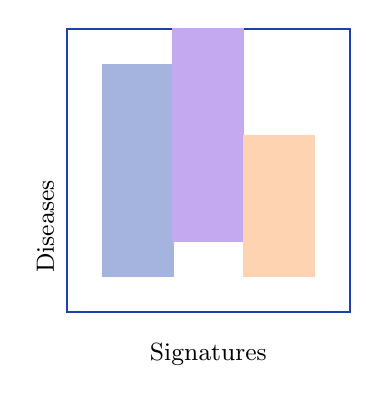
\begin{tikzpicture}[scale=0.9]
                \draw[thick, primaryblue] (0,0) -- (0,4) -- (4,4) -- (4,0) -- cycle;
                \node[below] at (2,-0.3) {\small Signatures};
                \node[left,rotate=90] at (-0.3,2) {\small Diseases};
                
                % Example heatmap cells
                \filldraw[primaryblue!40] (0.5,0.5) rectangle (1.5,3.5);
                \filldraw[accentpurple!40] (1.5,1,0) rectangle (2.5,4);
                \filldraw[warmorange!40] (2.5,0.5) rectangle (3.5,2.5);
            \end{tikzpicture}
            \vspace{0.5em}
            \small Signature-Disease Matrix
        \end{center}
    \end{columns}
\end{frame}

\begin{frame}{Genetic Discovery: PRS Enrichment in Signatures}
    \begin{block}{Key Findings}
        \begin{itemize}
            \item Cardiovascular PRS $\rightarrow$ strongly associated with metabolic signature
            \item Psychiatric PRS $\rightarrow$ associated with neuro/psychiatric signatures
            \item Genetic correlations reveal shared architecture
        \end{itemize}
    \end{block}
    
    \vspace{1em}
    
    \begin{center}
        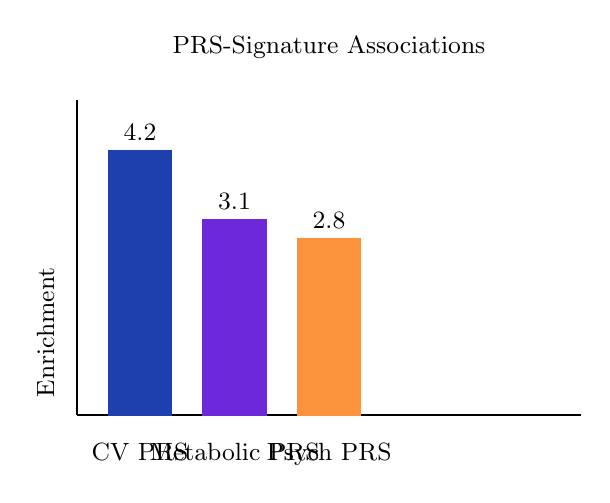
\begin{tikzpicture}[scale=0.8]
            % PRS bars
            \draw[thick] (0,0) -- (8,0);
            \draw[thick] (0,0) -- (0,5);
            
            % Example bars
            \filldraw[primaryblue] (0.5,0) rectangle (1.5,4.2);
            \node[above] at (1,4.2) {\small 4.2};
            \node[below] at (1,-0.3) {\small CV PRS};
            
            \filldraw[accentpurple] (2,0) rectangle (3,3.1);
            \node[above] at (2.5,3.1) {\small 3.1};
            \node[below] at (2.5,-0.3) {\small Metabolic PRS};
            
            \filldraw[warmorange] (3.5,0) rectangle (4.5,2.8);
            \node[above] at (4,2.8) {\small 2.8};
            \node[below] at (4,-0.3) {\small Psych PRS};
            
            \node[left,rotate=90] at (-0.5,2.5) {\small Enrichment};
            \node[above] at (4,5.5) {\small PRS-Signature Associations};
        \end{tikzpicture}
    \end{center}
    
    \vspace{0.5em}
    \begin{center}
        \textcolor{accentpurple}{\textbf{Signature-based GWAS reveals loci invisible to single-disease analyses}}
    \end{center}
\end{frame}

\begin{frame}{Prediction Performance: Outperforming Benchmarks}
    \begin{columns}
        \column{0.5\textwidth}
        \begin{block}{ASCVD Predictions}
            \begin{itemize}
                \item \textbf{10-year:} \aladyn{} 0.737 vs PCE 0.683
                \item[] \textcolor{accentpurple}{$\mathbf{+7.9\%}$ improvement}
                \item \textbf{30-year:} \aladyn{} 0.708 vs PREVENT 0.650
                \item[] \textcolor{accentpurple}{$\mathbf{+9.0\%}$ improvement}
            \end{itemize}
        \end{block}
        
        \begin{block}{vs Delphi-2M}
            \begin{itemize}
                \item Outperforms on 15/28 diseases
                \item Largest gains: Parkinson's (+35\%), CKD (+33\%)
            \end{itemize}
        \end{block}
        
        \column{0.5\textwidth}
        \begin{block}{vs Cox Baseline}
            \begin{itemize}
                \item Parkinson's: \textcolor{accentpurple}{+35.2\%}
                \item CKD: \textcolor{accentpurple}{+33.2\%}
                \item Stroke: \textcolor{accentpurple}{+31.6\%}
                \item ASCVD: \textcolor{accentpurple}{+16.3\%}
            \end{itemize}
        \end{block}
        
        \begin{exampleblock}{Dynamic Risk Assessment}
            Model updates predictions as patients age and develop conditions
        \end{exampleblock}
    \end{columns}
\end{frame}

\begin{frame}{The Bayesian Update in Action: Example Patient}
    \begin{columns}
        \column{0.5\textwidth}
        \begin{block}{Patient Timeline}
            \begin{itemize}
                \item Age 35: Enrollment
                \item Age 40: Hypertension
                \item Age 45: Type 2 Diabetes
                \item Age 50: Coronary Artery Disease
                \item Age 55: Ongoing monitoring
            \end{itemize}
        \end{block}
        
        \begin{block}{Signature Evolution}
            \begin{itemize}
                \item Metabolic signature loading increases over time
                \item Genetic predisposition (PRS) influences trajectory
                \item Risk predictions continuously updated
            \end{itemize}
        \end{block}
        
        \column{0.5\textwidth}
        \begin{center}
            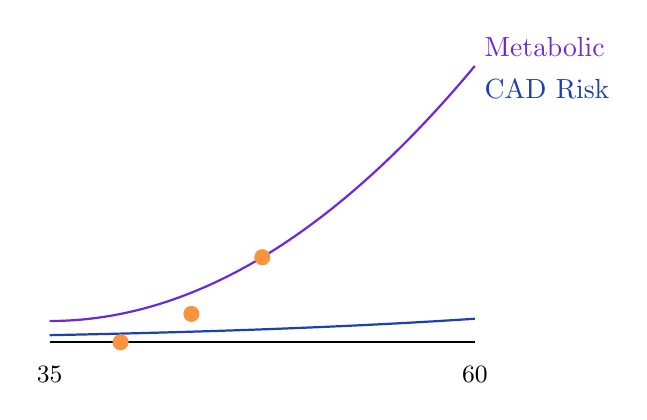
\begin{tikzpicture}[scale=0.9]
                % Time axis
                \draw[thick] (0,0) -- (6,0);
                \node[below] at (0,-0.2) {\small 35};
                \node[below] at (6,-0.2) {\small 60};
                
                % Signature trajectory
                \draw[smooth,thick,accentpurple] 
                    plot[domain=0:6,samples=100] (\x,{0.3 + 0.1*\x*\x});
                \node[above right,accentpurple] at (6,3.9) {Metabolic};
                
                % Disease probability
                \draw[smooth,thick,primaryblue] 
                    plot[domain=0:6,samples=100] (\x,{0.1*exp(0.2*\x)});
                \node[above right,primaryblue] at (6,3.3) {CAD Risk};
                
                % Events
                \filldraw[warmorange] (1,0) circle (3pt);
                \filldraw[warmorange] (2,0.4) circle (3pt);
                \filldraw[warmorange] (3,1.2) circle (3pt);
            \end{tikzpicture}
        \end{center}
    \end{columns}
    
    \vspace{1em}
    \begin{center}
        \textcolor{primaryblue}{\textbf{Posterior beliefs evolve as new information arrives}}
    \end{center}
\end{frame}

% ----------------------------------------------------------------------------
% SECTION: CONCLUSIONS
% ----------------------------------------------------------------------------
\section{Conclusions}

\begin{frame}{Key Takeaways}
    \begin{columns}
        \column{0.5\textwidth}
        \begin{block}{\faCheckCircle \quad Unified Framework}
            Simultaneous genomic discovery and clinical prediction
        \end{block}
        
        \begin{block}{\faDna \quad Interpretability}
            Signatures provide biological meaning through genetic architecture
        \end{block}
        
        \column{0.5\textwidth}
        \begin{block}{\faChartLine \quad Dynamic}
            Properly models lifetime risk evolution with Bayesian updating
        \end{block}
        
        \begin{block}{\faGlobe \quad Scalable}
            Works across diseases and biobanks
        \end{block}
    \end{columns}
    
    \vspace{2em}
    
    \begin{center}
        \Large
        \textcolor{accentpurple}{\textbf{Bayesian framework enables both discovery and prediction}}
    \end{center}
\end{frame}

\begin{frame}{Future Directions}
    \begin{columns}
        \column{0.5\textwidth}
        \begin{block}{Integration}
            \begin{itemize}
                \item Imaging (CAC, CT-coronary)
                \item AI-enhanced features (ECG, TTE)
                \item Multi-omics data
            \end{itemize}
        \end{block}
        
        \column{0.5\textwidth}
        \begin{block}{Applications}
            \begin{itemize}
                \item Intervention modeling (digital twins)
                \item Personalized screening
                \item Drug repurposing
            \end{itemize}
        \end{block}
    \end{columns}
    
    \vspace{2em}
    
    \begin{center}
        \Huge \faHeartbeat \quad \faCode \quad \faFlask
    \end{center}
\end{frame}

\begin{frame}[plain]
    \vfill
    \centering
    \Huge \textbf{Thank You!}
    
    \vspace{2em}
    
    \Large
    \textcolor{primaryblue}{\faEnvelope} \quad surbut@mgh.harvard.edu
    
    \vspace{1em}
    
    \large
    \textcolor{accentpurple}{\faGithub} \quad aladynoulli.hms.harvard.edu
    
    \vspace{3em}
    
    \normalsize
    \textit{Collaborators: P. Natarajan, G. Parmigiani, A. Gusev, and team}
    
    \vfill
\end{frame}

\end{document}
